\documentclass[tikz,border=10pt]{standalone}
\usetikzlibrary{calc}
\begin{document}
% Scale s=0.0077 cm/px, origin at circle centre O (px 543,538); y flipped
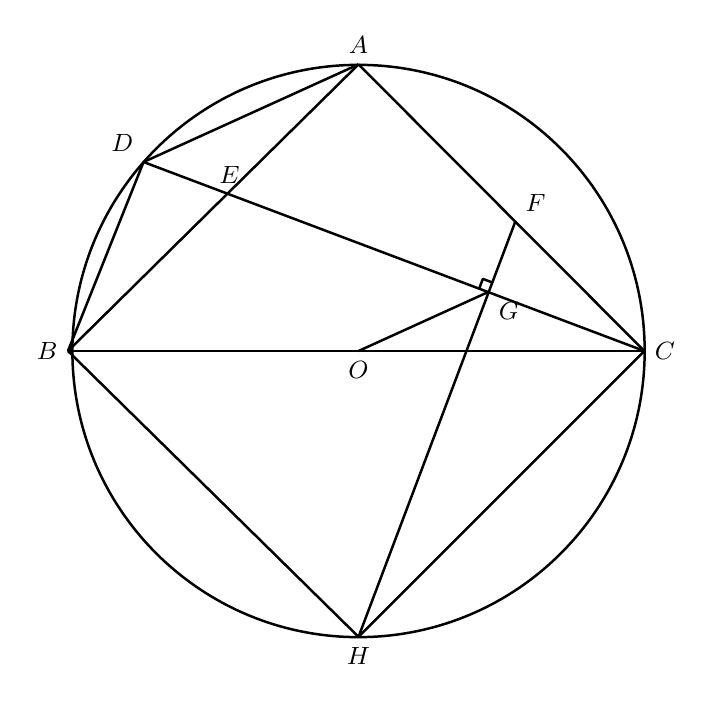
\begin{tikzpicture}[line width=0.9pt, line join=round,
  lbl/.style={font=\fontsize{9}{10.8}\selectfont}]

% Named points (converted from pixels)
\coordinate (O) at (0,0);
\coordinate (A) at (0,3.64);
\coordinate (B) at (-3.69,0);
\coordinate (C) at (3.63,0);
\coordinate (H) at (0,-3.63);
\coordinate (D) at (-2.73,2.40);
\coordinate (E) at (-1.64,1.99);
\coordinate (F) at (1.99,1.64);
\coordinate (G) at (1.65,0.75);
% Right-angle marker points
\coordinate (m1) at (1.534,0.797);
\coordinate (m2) at (1.579,0.916);
\coordinate (m3) at (1.698,0.871);

% Circle centred at O, radius 472 px
\draw (O) circle (3.634);

% Segments
\draw (B) -- (C);            % BC (diameter)
% (chord AH removed: not in original figure)
\draw (A) -- (B);
\draw (A) -- (C);
\draw (B) -- (H);
\draw (H) -- (C);
\draw (A) -- (D);
\draw (B) -- (D);
\draw (D) -- (C);            % passes through E and G
\draw (F) -- (H);            % passes through G
\draw (O) -- (G);

% Right angle at G between DC and FH
\draw (m1) -- (m2) -- (m3);

% Labels
\node[above, lbl] at (A) {$A$};
\node[left, lbl] at (B) {$B$};
\node[right, lbl] at (C) {$C$};
\node[below, lbl] at (H) {$H$};
\node[below, lbl] at (O) {$O$};
\node[above left, lbl] at (D) {$D$};
\node[above, lbl] at (E) {$E$};
\node[above right, lbl] at (F) {$F$};
\node[below right, lbl] at (G) {$G$};

\end{tikzpicture}
\end{document}